% Chapter 19: Sampling and Discretization
% IEEE-formatted LaTeX chapter for Control Systems Textbook
% Self-contained chapter - can be \input{} into main document

\chapter{Sampling and Discretization}
\label{ch:sampling_discretization}

\begin{abstract}
This chapter addresses the fundamental transition from continuous-time to discrete-time control systems. We trace the historical development from Nyquist's telegraph transmission work through Shannon's sampling theorem, derive the mathematical foundations of sampling and reconstruction, analyze aliasing phenomena, examine hold circuits, and present practical methods for discretizing continuous controllers. Laboratory experiments demonstrate aliasing visually and compare continuous versus discrete controller implementations.
\end{abstract}

%=============================================================================
\section{Historical Motivation: From Telegraph Lines to Digital Control}
\label{sec:sampling_history}
%=============================================================================

The mathematics of sampling did not emerge from abstract curiosity but from an intensely practical problem: how to transmit the maximum amount of information through telegraph and telephone lines with strictly limited bandwidth. The answers discovered in the early twentieth century now underpin every digital control system, audio device, and communication network.

\subsection{Harry Nyquist and Telegraph Transmission Theory (1928)}
\label{subsec:nyquist}

Harry Nyquist, a Swedish-American engineer at AT\&T Bell Telephone Laboratories, published a landmark paper in 1928 titled ``Certain Topics in Telegraph Transmission Theory.'' This work addressed a pressing industrial problem: the transcontinental telephone network required transmitting multiple telegraph signals simultaneously over a single wire pair, a technique called \textit{multiplexing}.

\subsubsection{The Problem: Bandwidth Is Expensive}

In the 1920s, laying copper telephone lines across the United States represented an enormous capital investment. Each additional wire pair cost thousands of dollars per mile. Engineers sought to maximize the information-carrying capacity of existing infrastructure. The critical question was:

\begin{quote}
\textit{Given a communication channel with bandwidth $W$ hertz, what is the maximum rate at which independent signal values can be transmitted?}
\end{quote}

Nyquist's analysis revealed a fundamental limit. He demonstrated that a channel of bandwidth $W$ could transmit at most $2W$ independent values (symbols) per second. Attempting to transmit faster would cause \textit{intersymbol interference}---successive symbols would blur together, becoming indistinguishable at the receiver.

\subsubsection{Nyquist's Key Insight}

Nyquist recognized that a bandlimited signal (one containing no frequencies above $W$ Hz) could be completely characterized by samples taken at rate $2W$ samples per second. More precisely, he showed that:

\begin{tcolorbox}[colback=blue!5!white,colframe=blue!75!black,title=Nyquist's Sampling Principle (1928)]
A signal containing no frequencies higher than $W$ hertz is completely determined by its values at uniformly spaced instants separated by $\dfrac{1}{2W}$ seconds.
\end{tcolorbox}

This result implied that sampling at twice the highest frequency component preserved all information in the original signal. Conversely, sampling slower than this rate would inevitably lose information---frequencies would become confused with one another, a phenomenon Nyquist understood but did not name.

\subsubsection{Impact on Multiplexing}

Nyquist's theorem enabled the design of time-division multiplexing systems. If each telephone voice channel occupied bandwidth $W = 4$ kHz (the standard telephone band), then $2W = 8000$ samples per second would suffice to capture all information. Multiple telephone conversations could share a single high-bandwidth channel by interleaving their samples in time---the birth of digital telephony, though the actual implementation would wait for digital electronics.

\subsection{Claude Shannon and the Sampling Theorem (1949)}
\label{subsec:shannon}

Claude Shannon, also at Bell Labs, formalized and extended Nyquist's work in his groundbreaking 1949 paper ``Communication in the Presence of Noise.'' Shannon provided the mathematical rigor that transformed Nyquist's engineering insight into a theorem with precise conditions and a reconstruction formula.

\subsubsection{Shannon's Formulation}

Shannon stated the sampling theorem in its now-standard form:

\begin{tcolorbox}[colback=green!5!white,colframe=green!75!black,title=Nyquist-Shannon Sampling Theorem]
If a function $x(t)$ contains no frequencies higher than $f_{\max}$ hertz, then it is completely determined by its values at a series of points spaced $\dfrac{1}{2f_{\max}}$ seconds apart. The original signal can be exactly reconstructed from these samples using the interpolation formula:
\begin{equation}
x(t) = \sum_{n=-\infty}^{\infty} x(nT) \, \mathrm{sinc}\left(\frac{t - nT}{T}\right)
\label{eq:shannon_reconstruction}
\end{equation}
where $T = \dfrac{1}{2f_{\max}}$ is the sampling period and $\mathrm{sinc}(u) = \dfrac{\sin(\pi u)}{\pi u}$.
\end{tcolorbox}

Shannon's contribution was not merely restating Nyquist but providing:
\begin{enumerate}
    \item A rigorous mathematical proof based on Fourier analysis
    \item An explicit reconstruction formula (the sinc interpolation)
    \item Connection to information theory and channel capacity
    \item Analysis of what happens when the conditions are violated (aliasing)
\end{enumerate}

\subsubsection{The Information Theory Context}

Shannon's sampling theorem appeared in his broader development of information theory. He recognized that sampling was not merely a practical convenience but a fundamental statement about information content. A bandlimited signal has a finite number of ``degrees of freedom'' per unit time, precisely $2W$ per second. Sampling captures exactly these degrees of freedom---no more, no less.

\subsection{The Problem That Drove the Mathematics}
\label{subsec:telephone_problem}

The telephone industry's central challenge was economic: voice communication required transmitting signals from approximately 300 Hz to 3400 Hz (the frequency range essential for speech intelligibility). This 3.1 kHz bandwidth, rounded to 4 kHz for engineering margin, could theoretically be represented by 8000 samples per second.

\subsubsection{Why Sampling?}

The advantage of sampling became apparent with the development of pulse-code modulation (PCM) at Bell Labs in the 1930s and 1940s. If each sample could be quantized to a finite number of levels (e.g., 256 levels using 8 bits), then voice could be transmitted as a sequence of numbers. These numbers offered:

\begin{itemize}
    \item \textbf{Regeneration}: Unlike analog signals that accumulate noise through repeaters, digital signals can be perfectly regenerated at each relay station
    \item \textbf{Multiplexing}: Multiple conversations can share a channel through time-division multiplexing
    \item \textbf{Storage}: Signals can be stored in digital memory
    \item \textbf{Processing}: Digital signal processing, filtering, and encryption become possible
\end{itemize}

\subsubsection{The Cost of Undersampling}

What happens if economic pressure leads engineers to sample below the Nyquist rate? Shannon's analysis revealed that frequencies above half the sampling rate would ``fold back'' into the baseband, appearing as spurious lower frequencies. This \textit{aliasing} effect corrupts the signal irreversibly---no subsequent processing can undo the damage.

\subsection{Early Digital Computers and Sampled-Data Systems}
\label{subsec:digital_computers}

The emergence of digital computers in the 1950s and 1960s created an entirely new domain for sampling theory: automatic control.

\subsubsection{Why Computers Cannot Handle Continuous Signals}

Digital computers are fundamentally discrete devices. They operate on finite sequences of numbers, perform calculations at discrete instants, and communicate through digital interfaces. When a computer must control a physical process---maintaining temperature in a chemical reactor, guiding a spacecraft, or positioning a machine tool---it confronts an inherent mismatch:

\begin{itemize}
    \item The physical world evolves continuously in time
    \item The computer operates at discrete instants
    \item Sensors produce continuous voltages that must be digitized
    \item Actuators require analog commands that must be synthesized from discrete values
\end{itemize}

This mismatch necessitated a complete theory of \textit{sampled-data control systems}.

\subsubsection{Radar Systems: Early Digital Control}

The first large-scale applications of digital control emerged in military radar and fire-control systems during World War II and the Cold War. The SAGE (Semi-Automatic Ground Environment) air defense system of the 1950s used digital computers to track aircraft based on radar returns sampled at discrete intervals. These systems required:

\begin{enumerate}
    \item Sampling radar signals at rates sufficient to track aircraft without aliasing their motion
    \item Implementing tracking filters (predecessors to the Kalman filter) in discrete time
    \item Generating smooth guidance commands from discrete computations
\end{enumerate}

\subsubsection{Aerospace Applications}

The Apollo guidance computer, operational in the 1960s, controlled spacecraft attitude and navigation using sampled sensor data and discrete control algorithms. With limited computational power (a 2 MHz clock, 2 KB of RAM), these systems had to carefully balance sample rate against computational burden---too fast sampling overwhelmed the processor; too slow sampling degraded control performance.

\subsubsection{Process Control}

Chemical plants, refineries, and power stations adopted digital control in the 1970s and 1980s. These applications typically involved relatively slow dynamics (time constants of minutes to hours) but required high reliability and the ability to coordinate hundreds of control loops. Digital systems offered programmability, data logging, and networked communication impossible with analog controllers.

\subsection{The Fundamental Question for Control Engineers}
\label{subsec:fundamental_question}

All these applications raised the same fundamental question:

\begin{tcolorbox}[colback=yellow!10!white,colframe=orange!75!black,title=The Digital Control Question]
Given a continuous-time system that must be controlled by a digital computer:
\begin{enumerate}
    \item How fast must we sample to preserve control performance?
    \item How do we convert continuous controller designs to discrete implementations?
    \item What artifacts arise from sampling, and how do we mitigate them?
\end{enumerate}
\end{tcolorbox}

The remainder of this chapter answers these questions with mathematical precision and practical guidance.

%=============================================================================
\section{Modern Applications of Sampling and Discretization}
\label{sec:modern_applications}
%=============================================================================

The principles established by Nyquist and Shannon now pervade every digital system that interacts with the analog world.

\subsection{Digital Audio}
\label{subsec:digital_audio}

The compact disc (CD), introduced in 1982, samples audio at 44.1 kHz with 16-bit resolution. This rate was chosen because:

\begin{itemize}
    \item Human hearing extends to approximately 20 kHz
    \item The Nyquist theorem requires sampling above 40 kHz
    \item A small margin (44.1 kHz) provides headroom for practical anti-aliasing filters
    \item The specific value 44.1 kHz aligned with existing video equipment standards
\end{itemize}

Modern high-resolution audio systems sample at 96 kHz, 192 kHz, or even higher---not because humans can hear frequencies above 20 kHz, but because higher sample rates ease anti-aliasing filter requirements and provide margin for signal processing.

\subsection{Digital Control in Microcontrollers}
\label{subsec:microcontroller_control}

Modern embedded systems implement control algorithms on microcontrollers with integrated analog-to-digital converters (ADCs) and pulse-width modulation (PWM) outputs. Typical applications include:

\begin{itemize}
    \item \textbf{Motor control}: Sample rates of 10--100 kHz for brushless DC motor commutation
    \item \textbf{Power electronics}: Switching converters operate at 50--500 kHz with control loops at 10--100 kHz
    \item \textbf{Automotive systems}: Engine control units sample sensors at 1--10 kHz
    \item \textbf{Consumer electronics}: Temperature control, battery management at 1--100 Hz
\end{itemize}

The sample rate selection involves tradeoffs between control bandwidth, computational load, sensor noise, and power consumption.

\subsection{Anti-Aliasing in Signal Processing}
\label{subsec:antialiasing}

Every properly designed data acquisition system includes an anti-aliasing filter before the analog-to-digital converter. This lowpass filter attenuates frequencies above half the sampling rate, preventing aliasing. Design considerations include:

\begin{itemize}
    \item Filter order (steeper cutoff requires higher-order filters)
    \item Phase distortion (important for time-domain applications)
    \item Cost and complexity tradeoffs
    \item Oversampling strategies that relax filter requirements
\end{itemize}

\subsection{Real-Time Embedded Systems}
\label{subsec:realtime}

In real-time control systems, the sample period establishes the fundamental timing constraint. All sensor reading, control computation, and actuator output must complete within each sample period. This creates design constraints:

\begin{equation}
T_{\text{computation}} + T_{\text{I/O}} < T_{\text{sample}}
\label{eq:realtime_constraint}
\end{equation}

Failure to meet this deadline can destabilize the control system or create unpredictable behavior. Real-time operating systems and careful software architecture ensure deterministic timing.

%=============================================================================
\section{Mathematical Foundations of Sampling}
\label{sec:math_foundations}
%=============================================================================

We now develop the complete mathematical framework for understanding sampling, aliasing, and reconstruction.

\subsection{The Ideal Sampling Process}
\label{subsec:ideal_sampling}

\subsubsection{Impulse Train Modulation}

The mathematical idealization of sampling treats the sampler as a modulator that multiplies the continuous signal by a train of impulses. Define the sampling period as $T$ and the sampling frequency as $f_s = 1/T$ (or $\omega_s = 2\pi f_s$ in radians per second).

The \textbf{impulse train} (Dirac comb) is:
\begin{equation}
\delta_T(t) = \sum_{n=-\infty}^{\infty} \delta(t - nT)
\label{eq:impulse_train}
\end{equation}

The \textbf{sampled signal} $x^*(t)$ is the product of the continuous signal $x(t)$ and the impulse train:
\begin{equation}
x^*(t) = x(t) \cdot \delta_T(t) = \sum_{n=-\infty}^{\infty} x(nT) \, \delta(t - nT)
\label{eq:sampled_signal}
\end{equation}

This represents a train of impulses whose amplitudes equal the signal values at the sampling instants.

\subsubsection{Frequency-Domain Analysis of Sampling}

The Fourier transform reveals the spectral effect of sampling. The impulse train has Fourier transform:
\begin{equation}
\mathcal{F}\{\delta_T(t)\} = \frac{1}{T} \sum_{k=-\infty}^{\infty} \delta(f - k f_s) = \frac{2\pi}{T} \sum_{k=-\infty}^{\infty} \delta(\omega - k\omega_s)
\label{eq:impulse_train_spectrum}
\end{equation}

Since multiplication in time corresponds to convolution in frequency:
\begin{equation}
X^*(f) = X(f) * \left( \frac{1}{T} \sum_{k=-\infty}^{\infty} \delta(f - k f_s) \right) = \frac{1}{T} \sum_{k=-\infty}^{\infty} X(f - k f_s)
\label{eq:sampled_spectrum}
\end{equation}

\begin{tcolorbox}[colback=green!5!white,colframe=green!75!black,title=Spectral Effect of Sampling]
Sampling creates infinitely many copies of the original spectrum $X(f)$, shifted to center frequencies $0, \pm f_s, \pm 2f_s, \ldots$, each scaled by $1/T$.
\end{tcolorbox}

\subsubsection{Visualization of the Sampled Spectrum}

Figure~\ref{fig:sampling_spectrum} illustrates this spectral replication.

\begin{figure}[htbp]
\centering
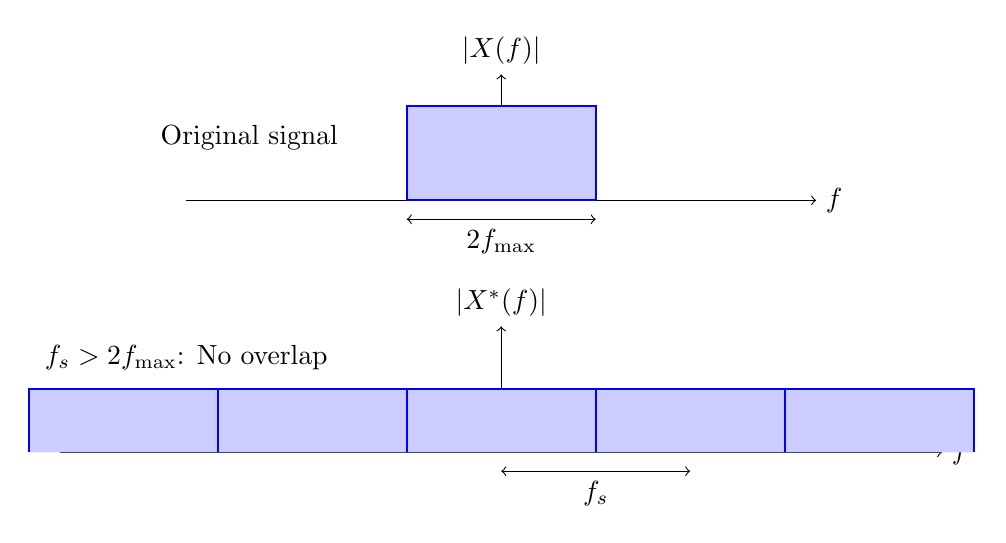
\begin{tikzpicture}[scale=0.8]
    % Original spectrum
    \begin{scope}[shift={(0,4)}]
        \draw[->] (-5,0) -- (5,0) node[right] {$f$};
        \draw[->] (0,0) -- (0,2) node[above] {$|X(f)|$};
        \draw[thick, blue, fill=blue!20] (-1.5,0) -- (-1.5,1.5) -- (0,1.5) -- (0,1.5) -- (1.5,1.5) -- (1.5,0) -- cycle;
        \draw[<->] (-1.5,-0.3) -- (1.5,-0.3) node[midway,below] {$2f_{\max}$};
        \node at (-4,1) {Original signal};
    \end{scope}

    % Sampled spectrum - proper sampling
    \begin{scope}[shift={(0,0)}]
        \draw[->] (-7,0) -- (7,0) node[right] {$f$};
        \draw[->] (0,0) -- (0,2) node[above] {$|X^*(f)|$};
        % Copies at -2fs, -fs, 0, fs, 2fs
        \foreach \k in {-2,-1,0,1,2} {
            \draw[thick, blue, fill=blue!20] (\k*3-1.5,0) -- (\k*3-1.5,1) -- (\k*3,1) -- (\k*3+1.5,1) -- (\k*3+1.5,0);
        }
        \draw[<->] (0,-0.3) -- (3,-0.3) node[midway,below] {$f_s$};
        \node at (-5,1.5) {$f_s > 2f_{\max}$: No overlap};
    \end{scope}
\end{tikzpicture}
\caption{Sampling in the frequency domain: the original spectrum is replicated at multiples of the sampling frequency $f_s$.}
\label{fig:sampling_spectrum}
\end{figure}

\subsection{The Nyquist-Shannon Sampling Theorem}
\label{subsec:nyquist_shannon}

\subsubsection{Statement of the Theorem}

\begin{theorem}[Nyquist-Shannon Sampling Theorem]
\label{thm:nyquist_shannon}
Let $x(t)$ be a bandlimited signal with no frequency components above $f_{\max}$ Hz:
\begin{equation}
X(f) = 0 \quad \text{for } |f| > f_{\max}
\label{eq:bandlimited}
\end{equation}
If $x(t)$ is sampled at rate $f_s > 2f_{\max}$, then $x(t)$ can be exactly reconstructed from its samples $\{x(nT)\}$ by the interpolation formula:
\begin{equation}
x(t) = \sum_{n=-\infty}^{\infty} x(nT) \, \mathrm{sinc}\left(\frac{t - nT}{T}\right)
\label{eq:sinc_interpolation}
\end{equation}
where $T = 1/f_s$ is the sampling period.
\end{theorem}

\subsubsection{Derivation from Frequency-Domain Analysis}

The proof proceeds by showing that an ideal lowpass filter can extract the original spectrum from the sampled spectrum.

\textbf{Step 1}: The sampled spectrum consists of shifted copies (Eq.~\ref{eq:sampled_spectrum}).

\textbf{Step 2}: If $f_s > 2f_{\max}$, adjacent copies do not overlap. The gap between the edge of one copy (at $f_{\max}$) and the nearest edge of the next copy (at $f_s - f_{\max}$) is:
\begin{equation}
\text{Gap} = (f_s - f_{\max}) - f_{\max} = f_s - 2f_{\max} > 0
\label{eq:gap}
\end{equation}

\textbf{Step 3}: An ideal lowpass filter with cutoff $f_c$ satisfying $f_{\max} < f_c < f_s - f_{\max}$ perfectly isolates the baseband copy centered at $f = 0$. Choosing $f_c = f_s/2$ (half the sampling frequency, the \textit{Nyquist frequency}):
\begin{equation}
H_{\text{ideal}}(f) = T \cdot \mathrm{rect}\left(\frac{f}{f_s}\right) =
\begin{cases}
T & |f| < f_s/2 \\
0 & |f| > f_s/2
\end{cases}
\label{eq:ideal_lpf}
\end{equation}

The factor $T$ compensates for the $1/T$ scaling introduced by sampling.

\textbf{Step 4}: The reconstructed spectrum is:
\begin{equation}
X_{\text{reconstructed}}(f) = X^*(f) \cdot H_{\text{ideal}}(f) = X(f)
\label{eq:reconstruction_spectrum}
\end{equation}

\textbf{Step 5}: The time-domain reconstruction filter is the inverse Fourier transform of $H_{\text{ideal}}(f)$:
\begin{equation}
h_{\text{ideal}}(t) = \mathrm{sinc}\left(\frac{t}{T}\right) = \frac{\sin(\pi t / T)}{\pi t / T}
\label{eq:sinc_impulse}
\end{equation}

Convolving the sampled signal with this sinc function yields the reconstruction formula (Eq.~\ref{eq:sinc_interpolation}).

\subsubsection{The Nyquist Frequency}

The \textbf{Nyquist frequency} $f_N = f_s/2$ is the highest frequency that can be unambiguously represented at sampling rate $f_s$. Equivalently, the \textbf{Nyquist rate} is the minimum sampling rate $2f_{\max}$ required to capture a signal with maximum frequency $f_{\max}$.

\subsection{Aliasing: When Sampling Fails}
\label{subsec:aliasing}

\subsubsection{The Aliasing Phenomenon}

When a signal contains frequencies above the Nyquist frequency ($f > f_s/2$), the spectral copies overlap. This overlap causes high-frequency components to ``fold back'' into the baseband, appearing as lower frequencies that are indistinguishable from legitimate signal components.

\begin{definition}[Aliasing]
\textbf{Aliasing} is the corruption of sampled data when frequency components above the Nyquist frequency fold into the baseband, creating spurious frequencies that cannot be separated from the true signal.
\end{definition}

\subsubsection{Mathematical Description of Folding}

Consider a sinusoidal signal at frequency $f_{\text{signal}}$ sampled at rate $f_s$. The sampled values are:
\begin{equation}
x(nT) = A \cos(2\pi f_{\text{signal}} \cdot nT + \phi) = A \cos\left(\frac{2\pi f_{\text{signal}}}{f_s} \cdot n + \phi\right)
\label{eq:sampled_sinusoid}
\end{equation}

Due to the periodicity of cosine with period $2\pi$, these samples are identical to those from a frequency:
\begin{equation}
f_{\text{alias}} = |f_{\text{signal}} - k \cdot f_s| \quad \text{for integer } k \text{ chosen so } 0 \leq f_{\text{alias}} \leq f_s/2
\label{eq:alias_frequency}
\end{equation}

\begin{tcolorbox}[colback=red!5!white,colframe=red!75!black,title=Aliasing Formula]
A signal at frequency $f$ sampled at rate $f_s$ produces the same samples as a signal at the \textbf{alias frequency}:
\begin{equation}
f_{\text{alias}} = \left| f - \left\lfloor \frac{f}{f_s} + 0.5 \right\rfloor \cdot f_s \right|
\label{eq:alias_formula}
\end{equation}
where $\lfloor \cdot \rfloor$ denotes rounding to the nearest integer.
\end{tcolorbox}

\subsubsection{Aliasing Examples}

\begin{example}[Simple Aliasing]
A 1200 Hz sinusoid is sampled at 1000 Hz. What frequency appears in the sampled data?

\textbf{Solution}: The signal frequency exceeds the Nyquist frequency (500 Hz). The alias frequency is:
\begin{equation*}
f_{\text{alias}} = |1200 - 1 \times 1000| = 200 \text{ Hz}
\end{equation*}

The sampled data appears to contain a 200 Hz signal, not 1200 Hz.
\end{example}

\begin{example}[Wagon Wheel Effect]
In film (24 frames per second), a wagon wheel with 12 spokes rotating at 25 revolutions per second appears to rotate slowly backward.

\textbf{Solution}: Each spoke passes a given position at rate $25 \times 12 = 300$ Hz. Sampled at 24 Hz, the alias frequency is:
\begin{equation*}
f_{\text{alias}} = |300 - 12 \times 24| = |300 - 288| = 12 \text{ Hz}
\end{equation*}

Since this aliases to 12 Hz but the sampling rate is 24 Hz, and $12 < 24/2 = 12$, the wheel appears to move at $12/12 = 1$ revolution per second---but in the opposite direction due to the phase reversal in folding.
\end{example}

\subsubsection{Frequency Domain Visualization of Aliasing}

Figure~\ref{fig:aliasing_spectrum} shows spectral overlap when $f_s < 2f_{\max}$.

\begin{figure}[htbp]
\centering
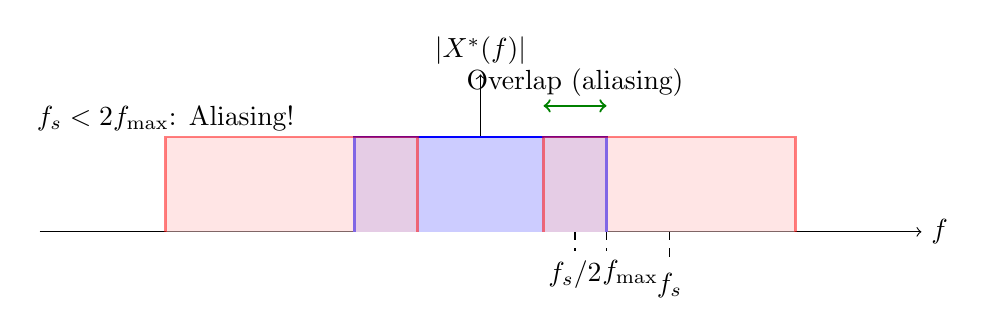
\begin{tikzpicture}[scale=0.8]
    % Aliased spectrum
    \draw[->] (-7,0) -- (7,0) node[right] {$f$};
    \draw[->] (0,0) -- (0,2.5) node[above] {$|X^*(f)|$};

    % Baseband copy
    \draw[thick, blue, fill=blue!20] (-2,0) -- (-2,1.5) -- (0,1.5) -- (2,1.5) -- (2,0);

    % Copy at +fs (overlapping)
    \draw[thick, red, fill=red!20, opacity=0.5] (1,0) -- (1,1.5) -- (3,1.5) -- (5,1.5) -- (5,0);

    % Copy at -fs (overlapping)
    \draw[thick, red, fill=red!20, opacity=0.5] (-5,0) -- (-5,1.5) -- (-3,1.5) -- (-1,1.5) -- (-1,0);

    % Indicate overlap region
    \draw[<->, thick, green!50!black] (1,2) -- (2,2);
    \node[above] at (1.5,2) {Overlap (aliasing)};

    % Labels
    \draw[dashed] (3,0) -- (3,-0.5) node[below] {$f_s$};
    \draw[dashed] (1.5,0) -- (1.5,-0.3) node[below] {$f_s/2$};
    \draw[dashed] (2,0) -- (2,-0.3) node[below, xshift=0.3cm] {$f_{\max}$};

    \node at (-5,1.8) {$f_s < 2f_{\max}$: Aliasing!};
\end{tikzpicture}
\caption{Aliasing in the frequency domain: when $f_s < 2f_{\max}$, spectral copies overlap, corrupting the baseband.}
\label{fig:aliasing_spectrum}
\end{figure}

\subsection{The Zero-Order Hold (ZOH)}
\label{subsec:zoh}

\subsubsection{Physical Motivation}

After sampling, the control computer calculates an output value. But digital-to-analog converters (DACs) produce continuous output---they cannot create impulses. The most common practical approach is the \textbf{zero-order hold} (ZOH): the DAC holds each output sample constant until the next sample arrives.

\begin{definition}[Zero-Order Hold]
The zero-order hold maintains the output value $y[n]$ constant from time $t = nT$ until time $t = (n+1)T$:
\begin{equation}
y(t) = y[n] \quad \text{for } nT \leq t < (n+1)T
\label{eq:zoh_definition}
\end{equation}
The resulting output is a staircase approximation to the ideal reconstructed signal.
\end{definition}

\subsubsection{Transfer Function of the ZOH}

The ZOH can be modeled as an LTI system with impulse response equal to a rectangular pulse of width $T$:
\begin{equation}
h_0(t) = \begin{cases}
1 & 0 \leq t < T \\
0 & \text{otherwise}
\end{cases}
\label{eq:zoh_impulse}
\end{equation}

Taking the Laplace transform:
\begin{equation}
H_0(s) = \int_0^T e^{-st} \, dt = \frac{1 - e^{-sT}}{s}
\label{eq:zoh_transfer}
\end{equation}

\begin{tcolorbox}[colback=green!5!white,colframe=green!75!black,title=Zero-Order Hold Transfer Function]
\begin{equation}
H_0(s) = \frac{1 - e^{-sT}}{s}
\label{eq:zoh_tf_boxed}
\end{equation}
This is a lowpass filter that introduces a delay of approximately $T/2$.
\end{tcolorbox}

\subsubsection{Frequency Response of the ZOH}

Substituting $s = j\omega$:
\begin{equation}
H_0(j\omega) = \frac{1 - e^{-j\omega T}}{j\omega} = e^{-j\omega T/2} \cdot \frac{e^{j\omega T/2} - e^{-j\omega T/2}}{j\omega}
\end{equation}
\begin{equation}
H_0(j\omega) = e^{-j\omega T/2} \cdot T \cdot \frac{\sin(\omega T/2)}{\omega T/2} = T \cdot \mathrm{sinc}\left(\frac{\omega T}{2\pi}\right) \cdot e^{-j\omega T/2}
\label{eq:zoh_frequency_response}
\end{equation}

The ZOH has:
\begin{itemize}
    \item \textbf{Magnitude}: Rolls off as a sinc function, with zeros at $\omega = 2\pi k/T$ ($k = 1, 2, \ldots$)
    \item \textbf{Phase}: A linear phase lag of $\omega T/2$, equivalent to a time delay of $T/2$
\end{itemize}

\subsubsection{Impact on Control Systems}

The ZOH delay of $T/2$ adds phase lag that can destabilize feedback systems. For a system with crossover frequency $\omega_c$, the additional phase lag is:
\begin{equation}
\phi_{\text{ZOH}} = -\frac{\omega_c T}{2} \quad \text{radians}
\label{eq:zoh_phase_lag}
\end{equation}

This motivates the rule of thumb: to limit ZOH-induced phase lag to a few degrees, the sampling frequency should be much higher than the control bandwidth.

\begin{figure}[htbp]
\centering
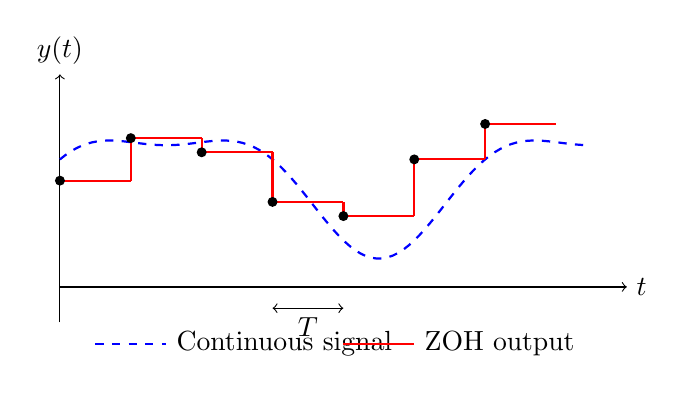
\begin{tikzpicture}[scale=0.9]
    % Time-domain ZOH visualization
    \draw[->] (0,0) -- (8,0) node[right] {$t$};
    \draw[->] (0,-0.5) -- (0,3) node[above] {$y(t)$};

    % Continuous signal (dashed)
    \draw[dashed, blue, thick, domain=0:7.5, samples=100] plot (\x, {1.5 + sin(\x*60)*0.8 + 0.3*cos(\x*120)});

    % ZOH reconstruction (staircase)
    \draw[thick, red] (0,1.5) -- (1,1.5);
    \draw[thick, red] (1,2.1) -- (2,2.1);
    \draw[thick, red] (2,1.9) -- (3,1.9);
    \draw[thick, red] (3,1.2) -- (4,1.2);
    \draw[thick, red] (4,1.0) -- (5,1.0);
    \draw[thick, red] (5,1.8) -- (6,1.8);
    \draw[thick, red] (6,2.3) -- (7,2.3);

    % Vertical transitions
    \foreach \x/\ya/\yb in {1/1.5/2.1, 2/2.1/1.9, 3/1.9/1.2, 4/1.2/1.0, 5/1.0/1.8, 6/1.8/2.3} {
        \draw[thick, red] (\x,\ya) -- (\x,\yb);
    }

    % Sample points
    \foreach \x/\y in {0/1.5, 1/2.1, 2/1.9, 3/1.2, 4/1.0, 5/1.8, 6/2.3} {
        \fill[black] (\x,\y) circle (2pt);
    }

    % Legend
    \draw[dashed, blue, thick] (0.5,-0.8) -- (1.5,-0.8) node[right, black] {Continuous signal};
    \draw[red, thick] (4,-0.8) -- (5,-0.8) node[right, black] {ZOH output};

    % Period annotation
    \draw[<->] (3,-0.3) -- (4,-0.3) node[midway, below] {$T$};
\end{tikzpicture}
\caption{Zero-order hold operation: the continuous signal (dashed) is sampled, and the ZOH maintains each sample value constant until the next sample.}
\label{fig:zoh_operation}
\end{figure}

\subsection{Discretization Methods for Controllers}
\label{subsec:discretization}

Given a continuous-time controller $C(s)$, we must convert it to a discrete-time controller $C(z)$ for implementation in a digital computer. Several methods exist, each with different accuracy and stability properties.

\subsubsection{Forward Euler (Forward Difference)}

The forward Euler method approximates the derivative by a forward difference:
\begin{equation}
\frac{dx}{dt} \approx \frac{x(t + T) - x(t)}{T} = \frac{x[n+1] - x[n]}{T}
\label{eq:forward_euler}
\end{equation}

In the Laplace/z-transform domains, $s \cdot X(s)$ corresponds to differentiation, and $z \cdot X(z)$ corresponds to a one-step advance. This gives the substitution:
\begin{equation}
\boxed{s \rightarrow \frac{z - 1}{T}}
\label{eq:forward_euler_substitution}
\end{equation}

\textbf{Properties}:
\begin{itemize}
    \item Simple to implement
    \item Can map stable continuous poles to unstable discrete poles
    \item Accuracy: $O(T)$
\end{itemize}

\subsubsection{Backward Euler (Backward Difference)}

The backward Euler method approximates the derivative by a backward difference:
\begin{equation}
\frac{dx}{dt} \approx \frac{x(t) - x(t - T)}{T} = \frac{x[n] - x[n-1]}{T}
\label{eq:backward_euler}
\end{equation}

This gives the substitution:
\begin{equation}
\boxed{s \rightarrow \frac{z - 1}{Tz}}
\label{eq:backward_euler_substitution}
\end{equation}

\textbf{Properties}:
\begin{itemize}
    \item Never maps stable continuous poles to unstable discrete poles (A-stable)
    \item May introduce excessive damping
    \item Accuracy: $O(T)$
\end{itemize}

\subsubsection{Tustin (Bilinear) Transform}

The Tustin method, also called the bilinear transform, uses the trapezoidal integration rule:
\begin{equation}
\int_{t-T}^{t} \frac{dx}{d\tau} \, d\tau \approx \frac{T}{2} \left[ \frac{dx}{dt}\bigg|_{t-T} + \frac{dx}{dt}\bigg|_t \right]
\label{eq:trapezoidal}
\end{equation}

This leads to the substitution:
\begin{equation}
\boxed{s \rightarrow \frac{2}{T} \cdot \frac{z - 1}{z + 1}}
\label{eq:tustin_substitution}
\end{equation}

\textbf{Properties}:
\begin{itemize}
    \item Maps the left half of the $s$-plane exactly to the interior of the unit circle in the $z$-plane
    \item Preserves stability: stable continuous systems yield stable discrete systems
    \item Introduces frequency warping: continuous frequency $\omega$ maps to discrete frequency $\omega_d = (2/T)\tan(\omega T/2)$
    \item Accuracy: $O(T^2)$
\end{itemize}

\begin{tcolorbox}[colback=blue!5!white,colframe=blue!75!black,title=Tustin Frequency Warping]
The Tustin transform maps continuous frequency $\omega$ to discrete frequency $\omega_d$ according to:
\begin{equation}
\omega_d = \frac{2}{T} \tan\left(\frac{\omega T}{2}\right)
\label{eq:frequency_warping}
\end{equation}
For $\omega T \ll 1$: $\omega_d \approx \omega$ (low frequency, good match).
As $\omega \rightarrow \omega_s/2$: $\omega_d \rightarrow \infty$ (high frequency compression).
\end{tcolorbox}

\subsubsection{Prewarping}

When a specific frequency (e.g., crossover frequency) must match exactly between continuous and discrete designs, \textit{prewarping} adjusts the Tustin transform:
\begin{equation}
s \rightarrow \frac{\omega_0}{\tan(\omega_0 T / 2)} \cdot \frac{z - 1}{z + 1}
\label{eq:prewarping}
\end{equation}

This ensures the continuous frequency $\omega_0$ maps exactly to the discrete frequency $\omega_0$.

\subsubsection{Zero-Order Hold Discretization (Exact Method)}

The most accurate discretization method accounts for the ZOH in the feedback loop. Given a continuous plant $G(s)$ with a ZOH on its input and a sampler on its output, the equivalent discrete transfer function is:
\begin{equation}
G(z) = (1 - z^{-1}) \mathcal{Z}\left\{ \frac{G(s)}{s} \right\}
\label{eq:zoh_discretization}
\end{equation}

where $\mathcal{Z}\{\cdot\}$ denotes the z-transform of the sampled step response.

This method is exact for the plant-hold combination but does not apply directly to controller discretization.

\subsubsection{Comparison of Discretization Methods}

Table~\ref{tab:discretization_comparison} summarizes the properties of each method.

\begin{table}[htbp]
\centering
\caption{Comparison of Discretization Methods}
\label{tab:discretization_comparison}
\begin{tabular}{|l|c|c|c|c|}
\hline
\textbf{Method} & \textbf{Substitution} & \textbf{Stability} & \textbf{Accuracy} & \textbf{Frequency} \\
\hline
Forward Euler & $\dfrac{z-1}{T}$ & May destabilize & $O(T)$ & Good at low $f$ \\[1.5ex]
\hline
Backward Euler & $\dfrac{z-1}{Tz}$ & Always stable & $O(T)$ & Over-damped \\[1.5ex]
\hline
Tustin & $\dfrac{2}{T}\dfrac{z-1}{z+1}$ & Preserves & $O(T^2)$ & Warped \\[1.5ex]
\hline
ZOH (plant) & Exact & Exact & Exact & Exact \\
\hline
\end{tabular}
\end{table}

\subsection{Choosing the Sample Rate}
\label{subsec:sample_rate_selection}

\subsubsection{Rule of Thumb}

For control systems, the sampling rate should be significantly higher than the Nyquist minimum to account for:
\begin{itemize}
    \item ZOH phase lag
    \item Computational delay
    \item Practical anti-aliasing filter limitations
    \item Margin for modeling errors
\end{itemize}

\begin{tcolorbox}[colback=yellow!10!white,colframe=orange!75!black,title=Sample Rate Guidelines]
For a control system with closed-loop bandwidth $\omega_{\text{BW}}$:
\begin{equation}
\omega_s \geq 10\omega_{\text{BW}} \quad \text{(minimum practical)}
\label{eq:sample_rate_min}
\end{equation}
\begin{equation}
\omega_s \approx 20\omega_{\text{BW}} \quad \text{(typical design)}
\label{eq:sample_rate_typical}
\end{equation}
Higher rates (30--50$\times$ bandwidth) may be needed for:
\begin{itemize}
    \item Systems with lightly damped resonances
    \item High-precision positioning
    \item Fast disturbance rejection
\end{itemize}
\end{tcolorbox}

\subsubsection{Tradeoffs in Sample Rate Selection}

\textbf{Benefits of higher sample rate}:
\begin{itemize}
    \item Better approximation of continuous control
    \item Reduced phase lag from ZOH
    \item Easier anti-aliasing filter design
    \item Better high-frequency disturbance rejection
\end{itemize}

\textbf{Costs of higher sample rate}:
\begin{itemize}
    \item Increased computational load
    \item More demanding real-time requirements
    \item Higher power consumption
    \item Increased data storage and communication bandwidth
\end{itemize}

%=============================================================================
\section{Practical Laboratory: Demonstrating Aliasing and Discretization Effects}
\label{sec:lab}
%=============================================================================

This laboratory provides hands-on experience with aliasing and discretization using readily available hardware.

\subsection{Learning Objectives}

Upon completion, students will be able to:
\begin{enumerate}
    \item Visually observe aliasing when a signal is undersampled
    \item Measure the alias frequency and verify the folding formula
    \item Discretize a continuous controller and compare performance
    \item Understand the effect of sample rate on control quality
\end{enumerate}

\subsection{Required Components}

\begin{table}[htbp]
\centering
\caption{Bill of Materials for Sampling Laboratory}
\label{tab:sampling_bom}
\begin{tabular}{|l|l|l|}
\hline
\textbf{Component} & \textbf{Specification} & \textbf{Qty} \\
\hline
Arduino Uno/Nano & ATmega328P & 1 \\
Function Generator & 0--100 kHz, sine output (or Arduino PWM + filter) & 1 \\
LEDs & Standard 5mm, assorted colors & 10 \\
Resistors & 220$\Omega$ for LEDs & 10 \\
Oscilloscope & Digital or analog, 2 channels & 1 \\
Lowpass Filter & RC filter components (10k$\Omega$, 0.1$\mu$F) & 1 set \\
Potentiometer & 10k$\Omega$ & 2 \\
DC Motor with Encoder & Same as Chapter 1 lab & 1 \\
Motor Driver & L298N or equivalent & 1 \\
\hline
\end{tabular}
\end{table}

\subsection{Experiment 1: Visualizing Aliasing}

\subsubsection{Setup}

This experiment demonstrates aliasing using a strobe-light approach. A row of LEDs represents the ``sampled'' output, while the true signal frequency is known.

\begin{enumerate}
    \item Wire 8 LEDs in a row, each controlled by a digital output pin
    \item Configure the Arduino to update the LED display at a fixed ``sample rate'' (e.g., 10 Hz)
    \item Generate a test signal using:
    \begin{itemize}
        \item A potentiometer rotated at controlled speed, or
        \item A function generator producing a low-frequency sine wave
    \end{itemize}
\end{enumerate}

\subsubsection{Software: Aliasing Demonstration}

\begin{lstlisting}[language=C++, caption={Aliasing Demonstration with LED Array}, label={lst:aliasing_demo}]
// Aliasing Demonstration
// Samples an analog input at adjustable rate and displays on LEDs

const int NUM_LEDS = 8;
const int LED_PINS[] = {2, 3, 4, 5, 6, 7, 8, 9};
const int ANALOG_PIN = A0;

// Sample rate control (adjustable via Serial)
unsigned long samplePeriodMs = 100;  // 10 Hz default
unsigned long lastSampleTime = 0;

void setup() {
    Serial.begin(115200);
    for (int i = 0; i < NUM_LEDS; i++) {
        pinMode(LED_PINS[i], OUTPUT);
    }
    Serial.println("Aliasing Demo - Enter sample period in ms:");
}

void displayOnLEDs(int value) {
    // Map 0-1023 to 0-7 (which LED to light)
    int ledIndex = map(value, 0, 1023, 0, NUM_LEDS - 1);

    // Turn off all LEDs, then light the selected one
    for (int i = 0; i < NUM_LEDS; i++) {
        digitalWrite(LED_PINS[i], (i == ledIndex) ? HIGH : LOW);
    }
}

void loop() {
    // Check for new sample period from Serial
    if (Serial.available()) {
        int newPeriod = Serial.parseInt();
        if (newPeriod > 0) {
            samplePeriodMs = newPeriod;
            Serial.print("Sample period set to ");
            Serial.print(samplePeriodMs);
            Serial.println(" ms");
        }
    }

    // Sample at the specified rate
    unsigned long now = millis();
    if (now - lastSampleTime >= samplePeriodMs) {
        lastSampleTime = now;

        int reading = analogRead(ANALOG_PIN);
        displayOnLEDs(reading);

        // Also output to Serial for plotting
        Serial.println(reading);
    }
}
\end{lstlisting}

\subsubsection{Procedure}

\begin{enumerate}
    \item \textbf{No aliasing}: Set the sample rate to 100 Hz (10 ms period). Slowly rotate the potentiometer (about 1 Hz). Observe that the LED display smoothly follows the rotation.

    \item \textbf{Introduce aliasing}: Reduce the sample rate to 2 Hz (500 ms period). Rotate the potentiometer at approximately 3 Hz. Observe that the LED display appears to move backward or erratically---this is aliasing.

    \item \textbf{Quantify aliasing}: With sample rate at 10 Hz, rotate the potentiometer at exactly 12 Hz (use a metronome or timer). The display should appear to move at 2 Hz ($|12 - 10| = 2$).

    \item \textbf{Nyquist limit}: Increase sample rate until the display correctly tracks the 12 Hz rotation. This should occur above 24 Hz.
\end{enumerate}

\subsubsection{Data Collection}

Complete Table~\ref{tab:aliasing_experiment}.

\begin{table}[htbp]
\centering
\caption{Aliasing Experiment Results}
\label{tab:aliasing_experiment}
\begin{tabular}{|c|c|c|c|}
\hline
\textbf{Signal Freq. (Hz)} & \textbf{Sample Rate (Hz)} & \textbf{Predicted Alias (Hz)} & \textbf{Observed (Hz)} \\
\hline
3 & 10 & 3 (no alias) & \\
\hline
8 & 10 & 2 & \\
\hline
12 & 10 & 2 & \\
\hline
15 & 10 & 5 & \\
\hline
18 & 10 & 2 & \\
\hline
12 & 30 & 12 (no alias) & \\
\hline
\end{tabular}
\end{table}

\subsection{Experiment 2: Effect of Sample Rate on Control Quality}

\subsubsection{Setup}

Using the motor control hardware from Chapter 1, implement a discrete PID controller at various sample rates.

\subsubsection{Software: Variable Sample Rate Controller}

\begin{lstlisting}[language=C++, caption={Variable Sample Rate Motor Control}, label={lst:variable_sample_rate}]
// Variable Sample Rate Motor Control
// Compare control quality at different sample rates

const int ENCODER_A = 2;
const int ENCODER_B = 3;
const int MOTOR_PWM1 = 5;
const int MOTOR_PWM2 = 6;

volatile long encoderCount = 0;
float setpoint = 0;

// PID gains (tune for 100 Hz operation first)
float Kp = 2.0;
float Ki = 0.5;
float Kd = 0.1;

// Sample period (adjustable)
unsigned long samplePeriodUs = 10000;  // 100 Hz default

// Control state
float integral = 0;
float prevError = 0;
unsigned long lastControlTime = 0;

// Performance metrics
unsigned long settlingStartTime = 0;
bool settled = false;
float maxOvershoot = 0;

void setup() {
    Serial.begin(115200);

    pinMode(ENCODER_A, INPUT_PULLUP);
    pinMode(ENCODER_B, INPUT_PULLUP);
    pinMode(MOTOR_PWM1, OUTPUT);
    pinMode(MOTOR_PWM2, OUTPUT);

    attachInterrupt(digitalPinToInterrupt(ENCODER_A),
                    updateEncoder, CHANGE);
    attachInterrupt(digitalPinToInterrupt(ENCODER_B),
                    updateEncoder, CHANGE);

    Serial.println("Variable Sample Rate Control");
    Serial.println("Commands: Snnn=setpoint, Tnnn=period(us)");
}

void updateEncoder() {
    // Same quadrature decoding as Chapter 1
    static int lastEncoded = 0;
    int MSB = digitalRead(ENCODER_A);
    int LSB = digitalRead(ENCODER_B);
    int encoded = (MSB << 1) | LSB;
    int sum = (lastEncoded << 2) | encoded;

    if (sum == 0b1101 || sum == 0b0100 ||
        sum == 0b0010 || sum == 0b1011) encoderCount++;
    if (sum == 0b1110 || sum == 0b0111 ||
        sum == 0b0001 || sum == 0b1000) encoderCount--;

    lastEncoded = encoded;
}

float getPositionDegrees() {
    const float COUNTS_PER_REV = 400.0;
    return (encoderCount / COUNTS_PER_REV) * 360.0;
}

void setMotorPWM(int pwm) {
    pwm = constrain(pwm, -255, 255);
    if (pwm > 0) {
        analogWrite(MOTOR_PWM1, pwm);
        analogWrite(MOTOR_PWM2, 0);
    } else {
        analogWrite(MOTOR_PWM1, 0);
        analogWrite(MOTOR_PWM2, -pwm);
    }
}

void loop() {
    // Parse commands
    if (Serial.available()) {
        char cmd = Serial.read();
        if (cmd == 'S' || cmd == 's') {
            setpoint = Serial.parseFloat();
            integral = 0;  // Reset integrator
            prevError = 0;
            settlingStartTime = micros();
            settled = false;
            maxOvershoot = 0;
            Serial.print("Setpoint: "); Serial.println(setpoint);
        } else if (cmd == 'T' || cmd == 't') {
            samplePeriodUs = Serial.parseInt();
            Serial.print("Sample period: ");
            Serial.print(samplePeriodUs);
            Serial.println(" us");
        }
    }

    // Control at specified sample rate
    unsigned long now = micros();
    if (now - lastControlTime >= samplePeriodUs) {
        float dt = (now - lastControlTime) / 1e6;
        lastControlTime = now;

        float position = getPositionDegrees();
        float error = setpoint - position;

        // PID calculation with proper discrete integration
        integral += error * dt;
        float derivative = (error - prevError) / dt;
        prevError = error;

        float output = Kp * error + Ki * integral + Kd * derivative;
        setMotorPWM((int)output);

        // Track performance metrics
        float overshoot = (setpoint > 0) ?
                          (position - setpoint) : (setpoint - position);
        if (overshoot > maxOvershoot) maxOvershoot = overshoot;

        if (!settled && abs(error) < 2.0) {
            settled = true;
            unsigned long settlingTime = now - settlingStartTime;
            Serial.print("Settled in ");
            Serial.print(settlingTime / 1000.0);
            Serial.print(" ms, Overshoot: ");
            Serial.println(maxOvershoot);
        }

        // Output for plotting
        Serial.print(setpoint); Serial.print(",");
        Serial.print(position); Serial.print(",");
        Serial.println(error);
    }
}
\end{lstlisting}

\subsubsection{Procedure}

\begin{enumerate}
    \item \textbf{Baseline (100 Hz)}: Set sample period to 10000 $\mu$s (100 Hz). Command a 90-degree step. Record settling time, overshoot, and steady-state error.

    \item \textbf{Reduce sample rate}: Test at 50 Hz, 20 Hz, 10 Hz, and 5 Hz. For each:
    \begin{itemize}
        \item Record settling time
        \item Record maximum overshoot
        \item Observe any oscillation or instability
    \end{itemize}

    \item \textbf{Increase sample rate}: Test at 200 Hz and 500 Hz. Note any improvement (or lack thereof due to other limiting factors).

    \item \textbf{Find the limit}: Reduce sample rate until the system becomes unstable. Record this critical sample rate.
\end{enumerate}

\subsubsection{Data Collection}

Complete Table~\ref{tab:sample_rate_experiment}.

\begin{table}[htbp]
\centering
\caption{Sample Rate Effect on Control Quality}
\label{tab:sample_rate_experiment}
\begin{tabular}{|c|c|c|c|c|}
\hline
\textbf{Sample Rate (Hz)} & \textbf{Settling Time (ms)} & \textbf{Overshoot (\%)} & \textbf{Oscillation?} & \textbf{Stable?} \\
\hline
500 & & & & \\
\hline
200 & & & & \\
\hline
100 & & & & \\
\hline
50 & & & & \\
\hline
20 & & & & \\
\hline
10 & & & & \\
\hline
5 & & & & \\
\hline
\end{tabular}
\end{table}

\subsection{Experiment 3: Comparing Discretization Methods}

\subsubsection{Objective}

Implement the same continuous PI controller using different discretization methods and compare transient response.

\subsubsection{Continuous PI Controller}

Consider the continuous PI controller:
\begin{equation}
C(s) = K_p + \frac{K_i}{s} = K_p \left(1 + \frac{1}{\tau_i s}\right)
\label{eq:lab_pi_continuous}
\end{equation}

with $K_p = 2.0$ and $K_i = 0.5$ (so $\tau_i = K_p/K_i = 4$).

\subsubsection{Discretized Controllers}

Using $T = 0.01$ s (100 Hz):

\textbf{Forward Euler} ($s \rightarrow (z-1)/T$):
\begin{equation}
C_{\text{FE}}(z) = K_p + \frac{K_i T}{z - 1} \quad \Rightarrow \quad u[n] = K_p e[n] + K_i T \sum_{k=0}^{n} e[k]
\end{equation}

\textbf{Backward Euler} ($s \rightarrow (z-1)/(Tz)$):
\begin{equation}
C_{\text{BE}}(z) = K_p + \frac{K_i T z}{z - 1} \quad \Rightarrow \quad u[n] = K_p e[n] + K_i T e[n] + u_i[n-1]
\end{equation}

\textbf{Tustin} ($s \rightarrow (2/T)(z-1)/(z+1)$):
\begin{equation}
C_{\text{Tustin}}(z) = K_p + \frac{K_i T}{2} \cdot \frac{z + 1}{z - 1}
\end{equation}

\subsubsection{Implementation}

\begin{lstlisting}[language=C++, caption={Comparing Discretization Methods}, label={lst:discretization_compare}]
// Discretization Method Comparison
// Select method via Serial: F=Forward Euler, B=Backward, T=Tustin

char discretizationMethod = 'T';  // Default: Tustin

// Integral state variables
float integralForward = 0;
float integralBackward = 0;
float integralTustin = 0;
float prevErrorTustin = 0;

float computePI(float error, float dt) {
    float proportional = Kp * error;
    float integralTerm = 0;

    switch (discretizationMethod) {
        case 'F':  // Forward Euler
            integralTerm = integralForward;
            integralForward += Ki * dt * error;
            break;

        case 'B':  // Backward Euler
            integralBackward += Ki * dt * error;
            integralTerm = integralBackward;
            break;

        case 'T':  // Tustin (Trapezoidal)
            integralTustin += Ki * dt * 0.5 * (error + prevErrorTustin);
            integralTerm = integralTustin;
            prevErrorTustin = error;
            break;
    }

    return proportional + integralTerm;
}

void resetIntegrators() {
    integralForward = 0;
    integralBackward = 0;
    integralTustin = 0;
    prevErrorTustin = 0;
}
\end{lstlisting}

\subsubsection{Procedure}

For each discretization method (Forward Euler, Backward Euler, Tustin):
\begin{enumerate}
    \item Reset integrators
    \item Command a step change in setpoint
    \item Record step response (position vs. time)
    \item Compare settling time, overshoot, and steady-state error
\end{enumerate}

At slow sample rates (e.g., 10 Hz), the differences between methods become more pronounced. At fast sample rates (e.g., 500 Hz), all methods should produce nearly identical results.

%=============================================================================
\section{Worked Examples}
\label{sec:examples}
%=============================================================================

\begin{example}[Minimum Sample Rate for Audio]
\label{ex:audio_sample_rate}
A digital audio system must capture human speech with frequencies from 300 Hz to 3400 Hz. What is the minimum theoretically required sample rate? What sample rate would you recommend in practice?

\textbf{Solution:}

The highest frequency component is $f_{\max} = 3400$ Hz.

By the Nyquist-Shannon theorem, the minimum sample rate is:
\begin{equation*}
f_{s,\min} = 2 f_{\max} = 2 \times 3400 = 6800 \text{ Hz}
\end{equation*}

In practice, we need margin for:
\begin{itemize}
    \item Anti-aliasing filter rolloff (practical filters cannot have infinite slope)
    \item Guard band to prevent any frequency folding
    \item Tolerance in component values
\end{itemize}

The telephone standard uses 8000 Hz, providing approximately 18\% margin. For higher quality, sample rates of 16 kHz (wideband telephony) or 44.1 kHz (CD audio) are used.

$\boxed{f_{s,\min} = 6800 \text{ Hz}; \quad \text{Practical: } f_s = 8000 \text{ Hz or higher}}$
\end{example}

\begin{example}[Identifying Aliased Frequency]
\label{ex:alias_identification}
A vibration sensor on a rotating machine samples at 1000 Hz. The machine has a shaft rotating at 630 RPM with a defect that creates a vibration at shaft frequency. An additional vibration appears in the data at 45 Hz. Could this be an alias? If so, what is the true frequency?

\textbf{Solution:}

Shaft frequency: $f_{\text{shaft}} = 630/60 = 10.5$ Hz.

Nyquist frequency: $f_N = f_s/2 = 500$ Hz.

Any true frequency $f_{\text{true}}$ that aliases to 45 Hz must satisfy:
\begin{equation*}
f_{\text{alias}} = |f_{\text{true}} - k \cdot f_s| = 45 \text{ Hz}
\end{equation*}

for some integer $k$. The possibilities are:
\begin{align*}
k = 0: \quad & f_{\text{true}} = 45 \text{ Hz} \\
k = 1: \quad & f_{\text{true}} = 1000 - 45 = 955 \text{ Hz, or } f_{\text{true}} = 1000 + 45 = 1045 \text{ Hz} \\
k = 2: \quad & f_{\text{true}} = 2000 - 45 = 1955 \text{ Hz, or } f_{\text{true}} = 2045 \text{ Hz} \\
& \vdots
\end{align*}

Checking if any are related to the shaft frequency:
\begin{itemize}
    \item $955/10.5 \approx 91$ (not an integer multiple)
    \item $1045/10.5 \approx 99.5$ (not an integer multiple)
    \item But $45/10.5 \approx 4.3$ (not exact either)
\end{itemize}

Let's check for blade-pass frequency. If the machine has 91 blades:
\begin{equation*}
f_{\text{blade}} = 91 \times 10.5 = 955.5 \text{ Hz}
\end{equation*}

This would alias to $|955.5 - 1000| = 44.5 \approx 45$ Hz.

$\boxed{\text{Yes, likely alias of 955 Hz (91$\times$ shaft frequency)}}$

\textbf{Verification}: Increase sample rate above 1910 Hz. If the 45 Hz peak moves or disappears and a peak near 955 Hz appears, aliasing is confirmed.
\end{example}

\begin{example}[Discretizing a First-Order System]
\label{ex:first_order_discretization}
Discretize the first-order lowpass filter $G(s) = \dfrac{1}{\tau s + 1}$ with $\tau = 0.1$ s using each discretization method. Use sample period $T = 0.02$ s (50 Hz).

\textbf{Solution:}

\textbf{Forward Euler} ($s \rightarrow (z-1)/T$):
\begin{equation*}
G_{\text{FE}}(z) = \frac{1}{\tau \cdot \frac{z-1}{T} + 1} = \frac{T}{\tau(z-1) + T} = \frac{T}{\tau z - \tau + T}
\end{equation*}
\begin{equation*}
G_{\text{FE}}(z) = \frac{0.02}{0.1z - 0.1 + 0.02} = \frac{0.02}{0.1z - 0.08} = \frac{0.2}{z - 0.8}
\end{equation*}

Pole at $z = 0.8$, which corresponds to continuous pole at $s = \ln(0.8)/T = -11.16$ rad/s (original: $s = -10$ rad/s).

\textbf{Backward Euler} ($s \rightarrow (z-1)/(Tz)$):
\begin{equation*}
G_{\text{BE}}(z) = \frac{1}{\tau \cdot \frac{z-1}{Tz} + 1} = \frac{Tz}{\tau(z-1) + Tz} = \frac{Tz}{\tau z - \tau + Tz}
\end{equation*}
\begin{equation*}
G_{\text{BE}}(z) = \frac{0.02z}{0.1z - 0.1 + 0.02z} = \frac{0.02z}{0.12z - 0.1} = \frac{0.167z}{z - 0.833}
\end{equation*}

Pole at $z = 0.833$, corresponding to $s = \ln(0.833)/T = -9.12$ rad/s (more damped than original).

\textbf{Tustin} ($s \rightarrow (2/T)(z-1)/(z+1)$):
\begin{equation*}
G_{\text{Tustin}}(z) = \frac{1}{\tau \cdot \frac{2}{T}\frac{z-1}{z+1} + 1} = \frac{z+1}{\frac{2\tau}{T}(z-1) + (z+1)}
\end{equation*}
\begin{equation*}
G_{\text{Tustin}}(z) = \frac{z+1}{10(z-1) + (z+1)} = \frac{z+1}{11z - 9} = \frac{z+1}{11(z - 0.818)}
\end{equation*}
\begin{equation*}
G_{\text{Tustin}}(z) = \frac{1}{11} \cdot \frac{z+1}{z - 0.818} = 0.091 \cdot \frac{z+1}{z - 0.818}
\end{equation*}

Pole at $z = 0.818$, corresponding to $s = \ln(0.818)/T = -10.05$ rad/s (very close to original).

\textbf{Comparison}:

\begin{center}
\begin{tabular}{|l|c|c|}
\hline
\textbf{Method} & \textbf{Discrete Pole} & \textbf{Equivalent Continuous Pole} \\
\hline
Forward Euler & 0.800 & -11.16 rad/s \\
Backward Euler & 0.833 & -9.12 rad/s \\
Tustin & 0.818 & -10.05 rad/s \\
\hline
Original & (exact: 0.819) & -10 rad/s \\
\hline
\end{tabular}
\end{center}

$\boxed{\text{Tustin most accurate; Forward Euler faster; Backward Euler slower}}$
\end{example}

\begin{example}[Designing an Anti-Aliasing Filter]
\label{ex:antialiasing_filter}
A data acquisition system samples at 10 kHz. Signals of interest are below 1 kHz. Design an anti-aliasing filter that attenuates the Nyquist frequency (5 kHz) by at least 40 dB.

\textbf{Solution:}

We need a lowpass filter with:
\begin{itemize}
    \item Passband: 0--1 kHz (signals of interest)
    \item Stopband: 5 kHz (must be attenuated by 40 dB)
\end{itemize}

The transition band ratio is:
\begin{equation*}
\text{Transition ratio} = \frac{f_{\text{stop}}}{f_{\text{pass}}} = \frac{5000}{1000} = 5
\end{equation*}

For a Butterworth filter, the attenuation at frequency $\omega$ is:
\begin{equation*}
|H(j\omega)|^2 = \frac{1}{1 + (\omega/\omega_c)^{2n}}
\end{equation*}

At the stopband edge, we require:
\begin{equation*}
20 \log_{10}|H(j\omega_{\text{stop}})| \leq -40 \text{ dB}
\end{equation*}
\begin{equation*}
|H|^2 \leq 10^{-4}
\end{equation*}
\begin{equation*}
\frac{1}{1 + (5)^{2n}} \leq 10^{-4}
\end{equation*}
\begin{equation*}
5^{2n} \geq 10^4 - 1 \approx 10^4
\end{equation*}
\begin{equation*}
2n \log(5) \geq 4
\end{equation*}
\begin{equation*}
n \geq \frac{4}{2 \times 0.699} = 2.86
\end{equation*}

A \textbf{third-order} Butterworth filter with cutoff at 1 kHz will provide approximately:
\begin{equation*}
\text{Attenuation at 5 kHz} = 10 \log_{10}(1 + 5^6) = 10 \log_{10}(15626) = 41.9 \text{ dB}
\end{equation*}

$\boxed{\text{Third-order Butterworth filter, } f_c = 1 \text{ kHz}}$

\textbf{Implementation}: Using an active Sallen-Key topology with op-amps, or a passive LC ladder for lower noise applications.
\end{example}

\begin{example}[ZOH Phase Lag Impact]
\label{ex:zoh_phase}
A continuous control system has crossover frequency $\omega_c = 100$ rad/s with phase margin 45 degrees. If this controller is implemented digitally with a ZOH, what is the maximum sample period to maintain at least 30 degrees of phase margin?

\textbf{Solution:}

The ZOH introduces phase lag of:
\begin{equation*}
\phi_{\text{ZOH}} = -\frac{\omega_c T}{2} \text{ radians} = -\frac{\omega_c T}{2} \times \frac{180}{\pi} \text{ degrees}
\end{equation*}

The original phase margin is 45 degrees. To maintain 30 degrees, we can lose at most:
\begin{equation*}
\Delta \phi = 45° - 30° = 15°
\end{equation*}

Setting the ZOH phase lag equal to 15 degrees:
\begin{equation*}
\frac{\omega_c T}{2} \times \frac{180}{\pi} = 15
\end{equation*}
\begin{equation*}
T = \frac{15 \times 2 \times \pi}{180 \times \omega_c} = \frac{30\pi}{180 \times 100} = \frac{\pi}{600} = 0.00524 \text{ s}
\end{equation*}

The sample rate is:
\begin{equation*}
f_s = \frac{1}{T} = \frac{600}{\pi} = 191 \text{ Hz}
\end{equation*}

The ratio of sample frequency to crossover frequency:
\begin{equation*}
\frac{f_s}{f_c} = \frac{191}{100/(2\pi)} = \frac{191 \times 2\pi}{100} = 12
\end{equation*}

$\boxed{T_{\max} = 5.24 \text{ ms}; \quad f_s \geq 191 \text{ Hz} \approx 12 \times f_c}$

This confirms the rule of thumb that $f_s \geq 10$--$20 \times f_c$ for adequate phase margin preservation.
\end{example}

\begin{example}[Complete Digital Controller Design]
\label{ex:complete_design}
A temperature control system has plant $G(s) = \dfrac{2}{10s + 1}$ (degrees per watt). Design a PI controller for zero steady-state error to step inputs. Then discretize using the Tustin method for implementation at 10 Hz.

\textbf{Solution:}

\textbf{Step 1: Continuous Controller Design}

For zero steady-state error to a step, we need a Type 1 system. The plant is Type 0, so the controller must include an integrator.

Choose a PI controller: $C(s) = K_p\left(1 + \dfrac{1}{\tau_i s}\right)$

The open-loop transfer function is:
\begin{equation*}
L(s) = K_p\left(1 + \frac{1}{\tau_i s}\right) \cdot \frac{2}{10s + 1} = \frac{2K_p(\tau_i s + 1)}{\tau_i s(10s + 1)}
\end{equation*}

Using pole-zero cancellation for simplicity, set $\tau_i = 10$ s to cancel the plant pole:
\begin{equation*}
L(s) = \frac{2K_p(10s + 1)}{10s(10s + 1)} = \frac{2K_p}{10s} = \frac{K_p}{5s}
\end{equation*}

For crossover at $\omega_c = 0.1$ rad/s (response time $\approx 10$ s):
\begin{equation*}
|L(j\omega_c)| = 1 \Rightarrow \frac{K_p}{5 \times 0.1} = 1 \Rightarrow K_p = 0.5
\end{equation*}

Final continuous controller:
\begin{equation*}
C(s) = 0.5\left(1 + \frac{1}{10s}\right) = 0.5 + \frac{0.05}{s} = \frac{0.5s + 0.05}{s}
\end{equation*}

\textbf{Step 2: Tustin Discretization}

With $T = 0.1$ s, substitute $s \rightarrow \dfrac{2}{T}\dfrac{z-1}{z+1} = 20\dfrac{z-1}{z+1}$:

\begin{equation*}
C(z) = \frac{0.5 \cdot 20\frac{z-1}{z+1} + 0.05}{20\frac{z-1}{z+1}}
\end{equation*}
\begin{equation*}
C(z) = \frac{10(z-1) + 0.05(z+1)}{20(z-1)} = \frac{10z - 10 + 0.05z + 0.05}{20(z-1)}
\end{equation*}
\begin{equation*}
C(z) = \frac{10.05z - 9.95}{20(z-1)} = \frac{10.05z - 9.95}{20z - 20}
\end{equation*}

Dividing numerator and denominator by 20:
\begin{equation*}
C(z) = \frac{0.5025z - 0.4975}{z - 1}
\end{equation*}

\textbf{Step 3: Difference Equation}

Cross-multiplying:
\begin{equation*}
U(z)(z - 1) = E(z)(0.5025z - 0.4975)
\end{equation*}
\begin{equation*}
u[n] - u[n-1] = 0.5025 \cdot e[n] - 0.4975 \cdot e[n-1]
\end{equation*}
\begin{equation*}
u[n] = u[n-1] + 0.5025 \cdot e[n] - 0.4975 \cdot e[n-1]
\end{equation*}

$\boxed{u[n] = u[n-1] + 0.5025 \, e[n] - 0.4975 \, e[n-1]}$

This is the velocity form of PI control, which avoids integrator windup issues.
\end{example}

%=============================================================================
\section{Figures for TikZ Implementation}
\label{sec:tikz}
%=============================================================================

\subsection{Figure: Sampling and Reconstruction Block Diagram}

\begin{figure}[htbp]
\centering
\begin{tikzpicture}[auto, node distance=2.5cm, >=latex']
    % Blocks
    \node [input] (input) {};
    \node [block, right of=input, node distance=2cm] (aaf) {Anti-alias Filter};
    \node [block, right of=aaf, node distance=3cm] (sampler) {Sampler $f_s$};
    \node [block, right of=sampler, node distance=3cm] (digital) {Digital Processing};
    \node [block, right of=digital, node distance=3cm] (dac) {ZOH (DAC)};
    \node [block, right of=dac, node distance=3cm] (recon) {Reconstruction Filter};
    \node [output, right of=recon, node distance=2cm] (output) {};

    % Connections
    \draw [->] (input) -- node[above, pos=0.3] {$x(t)$} (aaf);
    \draw [->] (aaf) -- (sampler);
    \draw [->] (sampler) -- node[above] {$x[n]$} (digital);
    \draw [->] (digital) -- node[above] {$y[n]$} (dac);
    \draw [->] (dac) -- (recon);
    \draw [->] (recon) -- node[above, pos=0.7] {$y(t)$} (output);

    % Clock signal
    \node [above of=sampler, node distance=1.5cm] (clock) {$T = 1/f_s$};
    \draw [dashed, ->] (clock) -- (sampler);
    \draw [dashed, ->] (clock) -| (dac);
\end{tikzpicture}
\caption{Complete sampling and reconstruction system showing anti-aliasing filter, sampler, digital processing, DAC (ZOH), and reconstruction filter.}
\label{fig:sampling_reconstruction}
\end{figure}

\subsection{Figure: Aliasing Time Domain}

\begin{figure}[htbp]
\centering
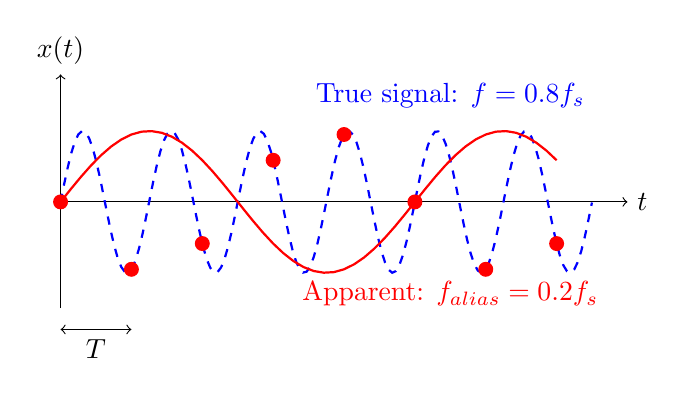
\begin{tikzpicture}[scale=0.9]
    % Axes
    \draw[->] (0,0) -- (8,0) node[right] {$t$};
    \draw[->] (0,-1.5) -- (0,1.8) node[above] {$x(t)$};

    % True high-frequency signal (dashed)
    \draw[dashed, blue, thick, domain=0:7.5, samples=150]
        plot (\x, {sin(\x*360*0.8)});

    % Sample points (at lower rate, showing aliasing)
    \foreach \t in {0, 1, 2, 3, 4, 5, 6, 7} {
        \pgfmathsetmacro{\y}{sin(\t*360*0.8)}
        \fill[red] (\t, \y) circle (3pt);
    }

    % Aliased low-frequency interpretation (solid)
    \draw[red, thick, domain=0:7, samples=50]
        plot (\x, {sin(\x*360*0.2)});

    % Legend
    \node[blue] at (5.5, 1.5) {True signal: $f = 0.8 f_s$};
    \node[red] at (5.5, -1.3) {Apparent: $f_{\text{alias}} = 0.2 f_s$};

    % Sample period annotation
    \draw[<->] (0,-1.8) -- (1,-1.8) node[midway, below] {$T$};
\end{tikzpicture}
\caption{Time-domain aliasing: a high-frequency signal (dashed blue) sampled below the Nyquist rate appears as a low-frequency signal (solid red) when reconstructed from the samples.}
\label{fig:aliasing_time_domain}
\end{figure}

\subsection{Figure: ZOH Step Response}

\begin{figure}[htbp]
\centering
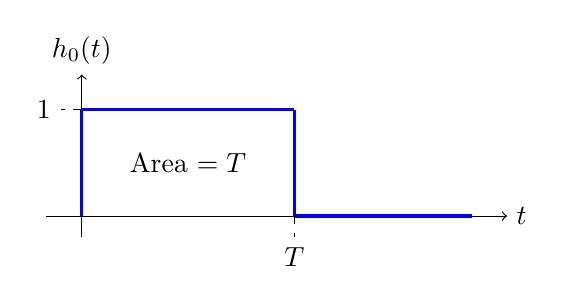
\begin{tikzpicture}[scale=0.9]
    % Axes
    \draw[->] (-0.5,0) -- (6,0) node[right] {$t$};
    \draw[->] (0,-0.3) -- (0,2) node[above] {$h_0(t)$};

    % ZOH impulse response (rectangular pulse)
    \draw[very thick, blue] (0,0) -- (0,1.5);
    \draw[very thick, blue] (0,1.5) -- (3,1.5);
    \draw[very thick, blue] (3,1.5) -- (3,0);
    \draw[very thick, blue] (3,0) -- (5.5,0);

    % Dashed lines for period
    \draw[dashed] (3,0) -- (3,-0.3) node[below] {$T$};
    \draw[dashed] (0,1.5) -- (-0.3,1.5) node[left] {$1$};

    % Labels
    \node at (1.5, 0.75) {Area $= T$};

\end{tikzpicture}
\caption{Impulse response of the zero-order hold: a rectangular pulse of height 1 and width $T$.}
\label{fig:zoh_impulse_response}
\end{figure}

\subsection{Figure: s-Plane to z-Plane Mapping}

\begin{figure}[htbp]
\centering
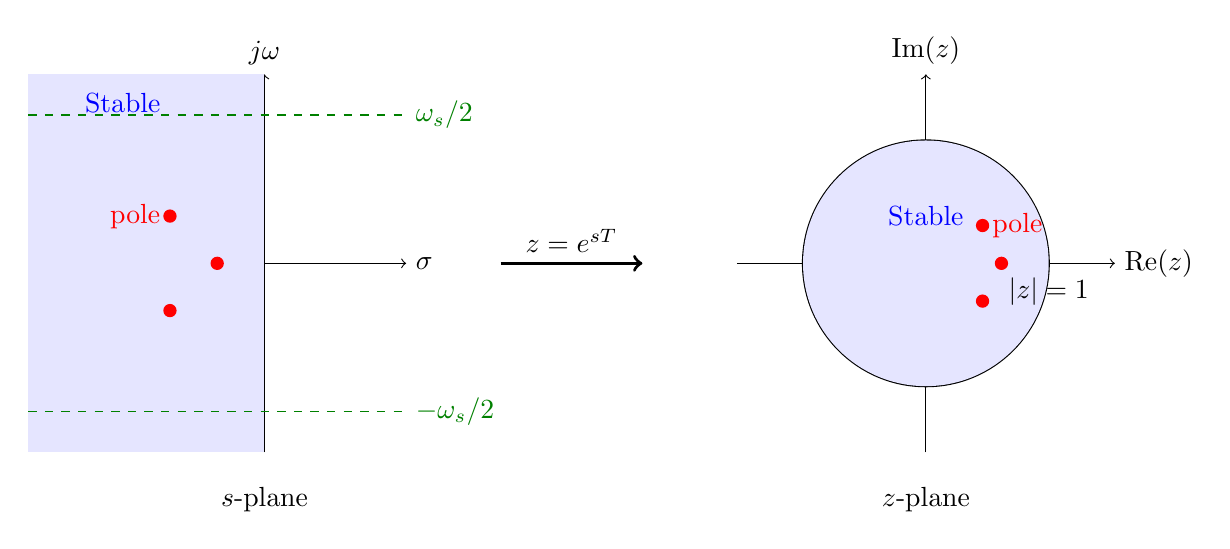
\begin{tikzpicture}[scale=1.2]
    % s-plane
    \begin{scope}[shift={(-3,0)}]
        \draw[->] (-2.5,0) -- (1.5,0) node[right] {$\sigma$};
        \draw[->] (0,-2) -- (0,2) node[above] {$j\omega$};

        % Stable region (shaded)
        \fill[blue!10] (-2.5,-2) rectangle (0,2);

        % Pole locations
        \fill[red] (-1, 0.5) circle (2pt) node[left] {pole};
        \fill[red] (-1, -0.5) circle (2pt);
        \fill[red] (-0.5, 0) circle (2pt);

        % Nyquist frequencies
        \draw[dashed, green!50!black] (-2.5, 1.57) -- (1.5, 1.57) node[right] {$\omega_s/2$};
        \draw[dashed, green!50!black] (-2.5, -1.57) -- (1.5, -1.57) node[right] {$-\omega_s/2$};

        \node at (0, -2.5) {$s$-plane};
        \node[blue] at (-1.5, 1.7) {Stable};
    \end{scope}

    % Arrow between planes
    \draw[->, very thick] (-0.5, 0) -- (1, 0) node[midway, above] {$z = e^{sT}$};

    % z-plane
    \begin{scope}[shift={(4,0)}]
        \draw[->] (-2,0) -- (2,0) node[right] {Re$(z)$};
        \draw[->] (0,-2) -- (0,2) node[above] {Im$(z)$};

        % Unit circle
        \draw[thick] (0,0) circle (1.3);

        % Stable region (shaded inside circle)
        \fill[blue!10] (0,0) circle (1.3);

        % Pole locations (mapped)
        \fill[red] (0.6, 0.4) circle (2pt) node[right] {pole};
        \fill[red] (0.6, -0.4) circle (2pt);
        \fill[red] (0.8, 0) circle (2pt);

        \node at (1.3, -0.3) {$|z|=1$};
        \node at (0, -2.5) {$z$-plane};
        \node[blue] at (0, 0.5) {Stable};
    \end{scope}
\end{tikzpicture}
\caption{Mapping from $s$-plane to $z$-plane: the left half-plane maps to the interior of the unit circle. The primary strip $|\omega| < \omega_s/2$ in the $s$-plane maps uniquely to the $z$-plane; additional strips (due to aliasing) fold onto the same region.}
\label{fig:s_to_z_mapping}
\end{figure}

%=============================================================================
\section{Chapter Summary}
\label{sec:summary}
%=============================================================================

This chapter established the theoretical and practical foundations for working with sampled-data control systems:

\begin{enumerate}
    \item \textbf{Historical Context}: Sampling theory emerged from the telephone industry's need to efficiently transmit voice signals. Nyquist (1928) established the fundamental rate limit; Shannon (1949) formalized the reconstruction theorem.

    \item \textbf{Nyquist-Shannon Theorem}: A bandlimited signal with no frequency content above $f_{\max}$ can be perfectly reconstructed from samples taken at rate $f_s > 2f_{\max}$.

    \item \textbf{Aliasing}: Sampling below the Nyquist rate causes high frequencies to fold into the baseband, creating spurious signals that cannot be distinguished from legitimate low-frequency content. Anti-aliasing filters prevent this.

    \item \textbf{Zero-Order Hold}: The ZOH maintains each sample constant until the next, creating a staircase approximation. It has transfer function $H_0(s) = (1 - e^{-sT})/s$ and introduces phase lag of approximately $\omega T/2$.

    \item \textbf{Discretization Methods}:
    \begin{itemize}
        \item Forward Euler: Simple but can destabilize
        \item Backward Euler: Always stable but over-damped
        \item Tustin: Best accuracy, preserves stability, but warps frequencies
        \item ZOH: Exact for plant with hold
    \end{itemize}

    \item \textbf{Sample Rate Selection}: For control systems, $f_s \geq 10$--$20 \times$ bandwidth provides adequate phase margin and discretization accuracy.
\end{enumerate}

\begin{tcolorbox}[colback=yellow!10!white,colframe=orange!75!black,title=Key Takeaway]
Sampling is not merely a practical convenience for digital implementation---it fundamentally transforms the system. Understanding aliasing, hold effects, and discretization accuracy is essential for designing digital controllers that achieve continuous-system performance. The Nyquist frequency represents an absolute information limit: frequencies above it cannot be captured, only corrupted.
\end{tcolorbox}

%=============================================================================
\section{Problems}
\label{sec:problems}
%=============================================================================

\begin{enumerate}
    \item \textbf{Nyquist Rate Calculation}: A control system must measure vibrations from 0.1 Hz to 250 Hz. What is the minimum sample rate? What would you recommend in practice?

    \item \textbf{Aliasing Identification}: A rotating shaft at 3600 RPM has 20 gear teeth. When sampled at 500 Hz, what frequency appears in the data? Is this aliased?

    \item \textbf{ZOH Analysis}: Calculate the magnitude and phase of the ZOH transfer function at $\omega = \omega_s/4$, $\omega_s/2$, and $\omega_s$. Sketch the Bode plot.

    \item \textbf{Discretization Comparison}: Discretize the controller $C(s) = \dfrac{s + 2}{s + 10}$ using Forward Euler, Backward Euler, and Tustin methods with $T = 0.05$ s. Compare pole locations.

    \item \textbf{Filter Design}: An ADC samples at 1 kHz. Design a second-order Butterworth anti-aliasing filter that attenuates the Nyquist frequency by at least 30 dB. Specify the cutoff frequency.

    \item \textbf{Phase Margin Preservation}: A continuous system has phase margin 60 degrees at crossover frequency 50 rad/s. What sample rate is needed to lose no more than 10 degrees to ZOH phase lag?

    \item \textbf{Tustin Prewarping}: A notch filter must have its zero exactly at 60 Hz when discretized at 1 kHz. Calculate the prewarped analog frequency.

    \item \textbf{Complete Design}: A motor has transfer function $G(s) = \dfrac{100}{s(s+10)}$. Design a continuous PI controller for 1 rad/s bandwidth, then discretize it using Tustin at 20 Hz. Write the difference equation.

    \item \textbf{Laboratory Analysis}: In Experiment 2, explain why the control system becomes unstable as sample rate decreases. What is the relationship between the critical sample rate and the closed-loop bandwidth?

    \item \textbf{Historical Reflection}: How did Nyquist's work on telegraph transmission lead to modern digital audio? Calculate the minimum bits per second required for telephone-quality voice (4 kHz bandwidth, 8-bit quantization).
\end{enumerate}

%=============================================================================
% End of Chapter
%=============================================================================
